\documentclass[12pt,]{book}
\usepackage{lmodern}
\usepackage{amssymb,amsmath}
\usepackage{ifxetex,ifluatex}
\usepackage{fixltx2e} % provides \textsubscript
\ifnum 0\ifxetex 1\fi\ifluatex 1\fi=0 % if pdftex
  \usepackage[T1]{fontenc}
  \usepackage[utf8]{inputenc}
\else % if luatex or xelatex
  \ifxetex
    \usepackage{mathspec}
  \else
    \usepackage{fontspec}
  \fi
  \defaultfontfeatures{Ligatures=TeX,Scale=MatchLowercase}
\fi
% use upquote if available, for straight quotes in verbatim environments
\IfFileExists{upquote.sty}{\usepackage{upquote}}{}
% use microtype if available
\IfFileExists{microtype.sty}{%
\usepackage{microtype}
\UseMicrotypeSet[protrusion]{basicmath} % disable protrusion for tt fonts
}{}
\usepackage[margin=1in]{geometry}
\usepackage{hyperref}
\hypersetup{unicode=true,
            pdftitle={A Guide to Nutrition and Food Security Assessments},
            pdfauthor={Ernest Guevarra},
            pdfborder={0 0 0},
            breaklinks=true}
\urlstyle{same}  % don't use monospace font for urls
\usepackage{natbib}
\bibliographystyle{apalike}
\usepackage{longtable,booktabs}
\usepackage{graphicx,grffile}
\makeatletter
\def\maxwidth{\ifdim\Gin@nat@width>\linewidth\linewidth\else\Gin@nat@width\fi}
\def\maxheight{\ifdim\Gin@nat@height>\textheight\textheight\else\Gin@nat@height\fi}
\makeatother
% Scale images if necessary, so that they will not overflow the page
% margins by default, and it is still possible to overwrite the defaults
% using explicit options in \includegraphics[width, height, ...]{}
\setkeys{Gin}{width=\maxwidth,height=\maxheight,keepaspectratio}
\IfFileExists{parskip.sty}{%
\usepackage{parskip}
}{% else
\setlength{\parindent}{0pt}
\setlength{\parskip}{6pt plus 2pt minus 1pt}
}
\setlength{\emergencystretch}{3em}  % prevent overfull lines
\providecommand{\tightlist}{%
  \setlength{\itemsep}{0pt}\setlength{\parskip}{0pt}}
\setcounter{secnumdepth}{5}
% Redefines (sub)paragraphs to behave more like sections
\ifx\paragraph\undefined\else
\let\oldparagraph\paragraph
\renewcommand{\paragraph}[1]{\oldparagraph{#1}\mbox{}}
\fi
\ifx\subparagraph\undefined\else
\let\oldsubparagraph\subparagraph
\renewcommand{\subparagraph}[1]{\oldsubparagraph{#1}\mbox{}}
\fi

%%% Use protect on footnotes to avoid problems with footnotes in titles
\let\rmarkdownfootnote\footnote%
\def\footnote{\protect\rmarkdownfootnote}

%%% Change title format to be more compact
\usepackage{titling}

% Create subtitle command for use in maketitle
\newcommand{\subtitle}[1]{
  \posttitle{
    \begin{center}\large#1\end{center}
    }
}

\setlength{\droptitle}{-2em}
  \title{A Guide to Nutrition and Food Security Assessments}
  \pretitle{\vspace{\droptitle}\centering\huge}
  \posttitle{\par}
  \author{Ernest Guevarra}
  \preauthor{\centering\large\emph}
  \postauthor{\par}
  \predate{\centering\large\emph}
  \postdate{\par}
  \date{05/03/2018}

\usepackage{booktabs}

\begin{document}
\maketitle

{
\setcounter{tocdepth}{1}
\tableofcontents
}
\hypertarget{introduction}{%
\chapter{Introduction}\label{introduction}}

\hypertarget{anthro1}{%
\chapter{Childhood undernutrition and anthropometry}\label{anthro1}}

Childhood undernutrition is an important global public health issue
contributing to nearly half of all deaths in children under 5 and is
widespread in Asia and Africa. This chapter discusses the various forms
of childhood undernutrition, describes the indices used to diagnose them
and the anthropometric measurements performed that will provide data to
calculate the various indices.

\hypertarget{forms-of-childhood-undernutrition}{%
\section{Forms of childhood
undernutrition}\label{forms-of-childhood-undernutrition}}

Childhood undernutrition manifests in various forms. It is important to
note the use of the term undernutrition rather than malnutrition as this
guide will not touch upon overweight and obesity. In this guide, the
focus will be on two forms of undernutrition: 1) acute undernutrition;
and, 2) chronic undernutrition. Childhood undernutrition manifested as
micronutrient deficiencies will not be discussed.

\hypertarget{acute-undernutrition}{%
\subsection{Acute undernutrition}\label{acute-undernutrition}}

Childhood \textbf{acute undernutrition} is a condition related to a
child's acute inadequate nutrition leading to rapid weight loss or
failure to gain weight normally. Situations such as acute shortage of
food and/or acute episodes of childhood illnesses such as diarrhoea,
acute respiratory infections and/or malaria can bring about this rapid
weight loss or weight gain failure in children.

\newpage

A. Physical signs and symptoms

Acute undernutrition in a child can manifest in two ways.

\begin{enumerate}
\def\labelenumi{\arabic{enumi}.}
\item
  \emph{Marasmus}: This condition is also called \emph{wasting} given
  that a child suffering from it presents as \emph{wasted} with an
  appearance of \emph{``skin and bones''} because of \emph{excessive
  thinness} that is due to rapid loss of muscle and fatty tissue. Other
  physical features include the child's face looking like an old man's
  (\emph{old man facies} due to loss of facial subcutaneous fat),
  child's rib cage is easily visible and skin folds on buttocks and
  thighs appearing like \emph{``baggy pants''}.
\item
  \emph{Kwashiorkor}: Some children with acute undernutrition develop
  \emph{nutritional oedema}. Oedema is an accumulation of fluid in the
  tissue, especially the feet and legs and nutritional oedema is
  specifically characterised as being \emph{bilateral and pitting}. The
  child with \emph{kwashiorkor} is \emph{withdrawn}, \emph{irritable},
  \emph{obviously ill} and \emph{will not eat}. The hair is thin, sparse
  and sometimes discoloured. The skin has symmetrical discoloured
  patches where the skin later cracks and peels off.
\end{enumerate}

\begin{figure}
\centering
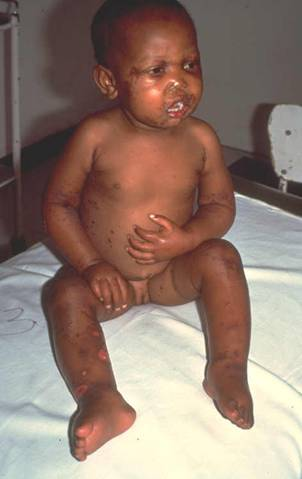
\includegraphics{images/oedema01.jpg}
\caption{Child with Bilateral oedema, skin and hair changes}
\end{figure}

\begin{figure}
\centering
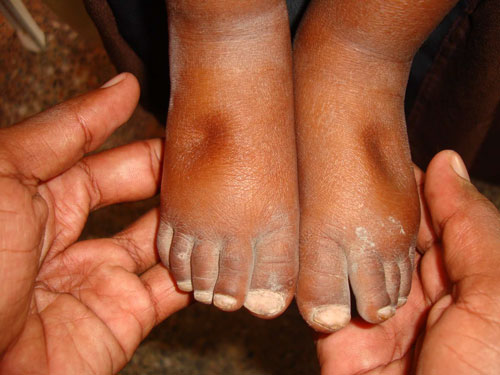
\includegraphics{images/oedema02.jpg}
\caption{Bilateral pitting oedeam}
\end{figure}

B. Anthropometric indices

The physical signs and symptoms of acute undernutrition described above
are considered pathognomonic of the condition i.e., if these signs and
symptoms are found in a child, it is very likley that the child has
acute undernutrition. However, other than physical signs, there are
anthropometric indices used to diagnose acute undernutrition in
children.

\begin{enumerate}
\def\labelenumi{\arabic{enumi}.}
\tightlist
\item
  Weight-for-height/weight-for-length
\end{enumerate}

The first independent criteria for \emph{marasmus} or \emph{wasting} is
weight-for-height (WFH)/weight-for-length (WFL). Given \emph{child A},
this child's weight is assessed against the mean weight of a standard
group of children in good health with the same height or length as
\emph{child A} (length is measured when the child is \textless{} 85 cms
in height or \textless{} 24 months old). \emph{Child A} is expected to
have a weight close to the mean weight of the standard group of healthy
children if \emph{child A} is also healthy and is not undernourished.
However, if \emph{child A}'s weight deviates significantly farther from
the mean weight of the standard group of healthy children, \emph{child
A} is considered to have low weight for its height and therefore
considered \emph{marasmic} or \emph{wasted}. This deviation from the
mean, also called \emph{standard deviation (SD)} in statistics, is
calculated for each child whose weight and height have been measured and
is expressed in terms of \emph{z-scores}. Therefore, the anthropometric
index used for \emph{wasting} is weight-for-height z-scores (WHZ) and
classification of level of wasting is done based on the following WHZ
cut-offs:

~

\begin{longtable}[]{@{}ll@{}}
\toprule
\begin{minipage}[b]{0.34\columnwidth}\raggedright
\textbf{WHZ}\strut
\end{minipage} & \begin{minipage}[b]{0.47\columnwidth}\raggedright
\textbf{Classification}\strut
\end{minipage}\tabularnewline
\midrule
\endhead
\begin{minipage}[t]{0.34\columnwidth}\raggedright
WHZ \textless{} -2SD\strut
\end{minipage} & \begin{minipage}[t]{0.47\columnwidth}\raggedright
Global Acute malnurition (GAM)\strut
\end{minipage}\tabularnewline
\begin{minipage}[t]{0.34\columnwidth}\raggedright
-3SD \(\geq\) WHZ \textless{} -2SD\strut
\end{minipage} & \begin{minipage}[t]{0.47\columnwidth}\raggedright
Moderate acute malnutrition (MAM)\strut
\end{minipage}\tabularnewline
\begin{minipage}[t]{0.34\columnwidth}\raggedright
WHZ \textless{} -3SD\strut
\end{minipage} & \begin{minipage}[t]{0.47\columnwidth}\raggedright
Severe acute malnutrition (SAM)\strut
\end{minipage}\tabularnewline
\bottomrule
\end{longtable}

\begin{enumerate}
\def\labelenumi{\arabic{enumi}.}
\setcounter{enumi}{1}
\tightlist
\item
  Mid-upper arm circumference
\end{enumerate}

The other independent criteria for \emph{marasmus} or \emph{wasting} is
the \emph{mid-upper arm circumference} or \emph{MUAC}. \emph{MUAC} is a
measure of muscle mass and therefore detects loss of muscle mass due to
wasting. \emph{MUAC} is a good predictor of mortality and in many
studies, \emph{MUAC} predicted death in children better than any other
anthropometric indicator. Unlike weight-for-height, \emph{MUAC} is used
as an anthropometric index without need for standardisation. The
\emph{MUAC} cut-offs used to classify a child as being \emph{marasmic}
or \emph{wasted} are:

~

\begin{longtable}[]{@{}ll@{}}
\toprule
\begin{minipage}[b]{0.34\columnwidth}\raggedright
\textbf{MUAC (mm)}\strut
\end{minipage} & \begin{minipage}[b]{0.47\columnwidth}\raggedright
\textbf{Classification}\strut
\end{minipage}\tabularnewline
\midrule
\endhead
\begin{minipage}[t]{0.34\columnwidth}\raggedright
MUAC \textless{} 125\strut
\end{minipage} & \begin{minipage}[t]{0.47\columnwidth}\raggedright
Global Acute malnurition (GAM)\strut
\end{minipage}\tabularnewline
\begin{minipage}[t]{0.34\columnwidth}\raggedright
115 \(\geq\) MUAC \textless{} 125\strut
\end{minipage} & \begin{minipage}[t]{0.47\columnwidth}\raggedright
Moderate acute malnutrition (MAM)\strut
\end{minipage}\tabularnewline
\begin{minipage}[t]{0.34\columnwidth}\raggedright
MUAC \textless{} 115\strut
\end{minipage} & \begin{minipage}[t]{0.47\columnwidth}\raggedright
Severe acute malnutrition (SAM)\strut
\end{minipage}\tabularnewline
\bottomrule
\end{longtable}

\begin{enumerate}
\def\labelenumi{\arabic{enumi}.}
\setcounter{enumi}{2}
\tightlist
\item
  Oedema test
\end{enumerate}

The final index for acute undernutrition is \emph{oedema testing} for
\emph{kwarshiorkor} cases. This test checks whether \emph{oedema} is
present and whether it is \emph{bilateral} and \emph{pitting}. Any sign
of bilateral pitting oedema, regardless of WHZ or MUAC classification,
is considered \emph{severe acute malnutrition}.

\hypertarget{chronic-undernutrition}{%
\subsection{Chronic undernutrition}\label{chronic-undernutrition}}

Childhood \textbf{chronic undernutrition} is a condition related to a
child's exposure to inadequate nutrition over a long period of time
leading to failure of linear growth. Stunted growth reflects a process
of failure to reach linear growth potential as a result of suboptimal
health and/or nutritional conditions.

~

A. Physical signs and symptoms

A child suffering from chronic undernutrition is also called
\emph{stunting/stunted}. Such a child is said to be short for its age
(see below).

~

B. Anthropometric indices

Like with acute undernutrition, an index is used to classify whether a
child has chronic malnutrition or not. This index is called
height-for-age (HFA) or length-for-age (LFA). Given \emph{child B}, this
child's length/height is assessed against the mean length/height of a
standard group of children in good health with the same age as
\emph{child B}. \emph{Child B} is expected to have a length/height close
to the mean length/height of the standard group of healthy children if
\emph{child B} is also health and well-nourished. However, if
\emph{child B}'s length/height deviates significantly farther from the
mean height of the standard group of healthy children, \emph{child B} is
considered to have low height for its age and therefore considered to be
\emph{stunting} or \emph{stunted}. This deviation from the mean, also
called \emph{standard deviation (SD)} in statistics, is calculated for
each child whose height has been measured and is expressed in terms of
\emph{z-scores}. Therefore, the anthropometric index used for
\emph{stunting/stuntedness} is height-for-age z-scores (HAZ) and
classification of level of stunting/stuntedness is done based on the
following WHZ cut-offs:

~

\begin{longtable}[]{@{}ll@{}}
\toprule
\begin{minipage}[b]{0.34\columnwidth}\raggedright
\textbf{HAZ}\strut
\end{minipage} & \begin{minipage}[b]{0.47\columnwidth}\raggedright
\textbf{Classification}\strut
\end{minipage}\tabularnewline
\midrule
\endhead
\begin{minipage}[t]{0.34\columnwidth}\raggedright
HAZ \textless{} -2SD\strut
\end{minipage} & \begin{minipage}[t]{0.47\columnwidth}\raggedright
Global stunting/stuntedness\strut
\end{minipage}\tabularnewline
\begin{minipage}[t]{0.34\columnwidth}\raggedright
-3SD \(\geq\) HAZ \textless{} -2SD\strut
\end{minipage} & \begin{minipage}[t]{0.47\columnwidth}\raggedright
Moderate stunting/stuntedness\strut
\end{minipage}\tabularnewline
\begin{minipage}[t]{0.34\columnwidth}\raggedright
HAZ \textless{} -3SD\strut
\end{minipage} & \begin{minipage}[t]{0.47\columnwidth}\raggedright
Severe stunting/stuntedness\strut
\end{minipage}\tabularnewline
\bottomrule
\end{longtable}

\hypertarget{anthro2}{%
\chapter{Performing anthropometric measurements}\label{anthro2}}

As described in \protect\hyperlink{anthro1}{Chapter 2}, to be able to
assess the anthropometric indices for acute and chronic undernutrition
four (4) anthropometric measurements needs to be collected: 1)
\emph{weight}; 2) \emph{height}; 3) \emph{mid-upper arm circumference
(MUAC)}; and, 4) \emph{oedema}. In addition to these anthropometric
measurements, information on the child's \emph{age (in months)} and
\emph{sex} will also be needed to be able to determine the appropriate
reference standards to use in calculating the child's corresponding
anthropometric indices. This chapter provides detailed directions on how
to perform anthropometric measurements accurately.

\hypertarget{measuring-weight}{%
\section{Measuring weight}\label{measuring-weight}}

\hypertarget{equipment-weighing-scales}{%
\subsection{Equipment: Weighing
scales}\label{equipment-weighing-scales}}

A. Types of weighing scales

Various types of scales are available to measure the weight of a child:
1) \emph{spring scales}; 2) \emph{hanging scales}; 2) \emph{beam balance
scales}; and, 3) \emph{digital scales}.

\emph{Spring scales} are the most common type of scales used worldwide.
\emph{Hanging scales} are a kind of \emph{spring scale} that is hung
from a height instead of laid flat on the ground. \emph{Hanging scales}
are commonly preferred in many countries because they can be transported
easily, can be used in almost any setting (particularly where a flat
surface is not available) and are relatively inexpensive. However, they
are not very accurate and as such are not recommended for use in
nutrition surveys.

\begin{figure}
\centering
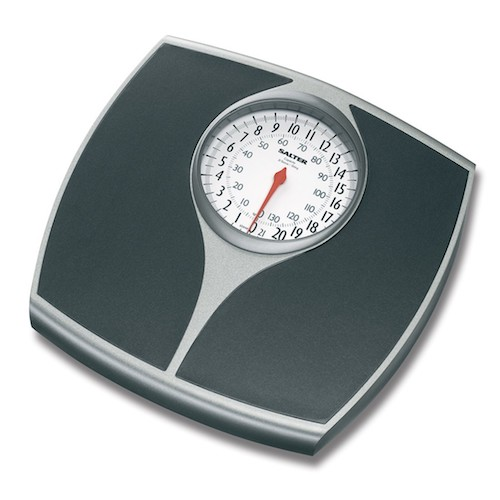
\includegraphics{images/springScale.jpg}
\caption{Bathroom scale (spring)}
\end{figure}

~

\begin{figure}
\centering
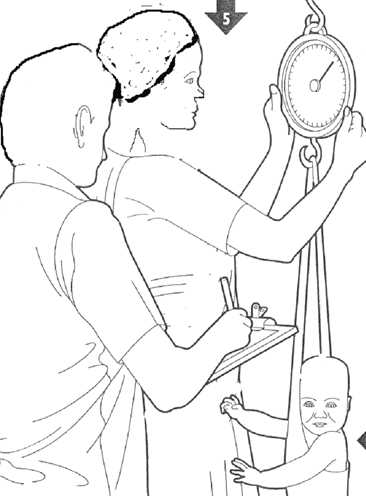
\includegraphics{images/hangingScale.png}
\caption{Hanging scale (spring)}
\end{figure}

~

\emph{Balance beam scales} are commonly used in health centers, as they
need to be positioned on a flat surface for accurate measurement and are
not easily transported.

\begin{figure}
\centering
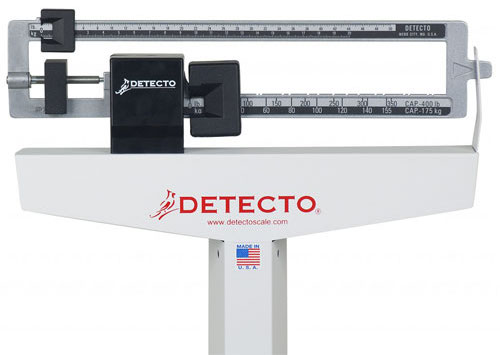
\includegraphics{images/balanceBeam.jpg}
\caption{Balance beam scales}
\end{figure}

\emph{Digital scales} on the other hand are highly accurate (for as long
as it is powered adequately and consistently), easily transportable
though requiring a flat surface on which to be laid upon. They are
generally of high quality and rugged for frequent field use as is needed
for a nutrition survey. This is why \emph{digital scales} are what's
currently recommended for use in anthropometric measurements in a field
survey setting.

In addition to being a \emph{digital scale}, it is recommended to weigh
children using a scale with the following features:

\begin{itemize}
\item
  Solidly built and durable
\item
  Electronic (digital reading)
\item
  Measures up to 150 kg
\item
  Measures to a precision of 0.1 kg (100g)
\item
  Allows tared weighing
\end{itemize}

\textbf{``Tared weighing''} means that the scale can be re-set to zero
(\emph{``tared''}) with the person just weighed still on it. Thus, a
mother can stand on the scale, be weighed, and the scale tared. While
remaining on the scale, if she is given her child to hold, the child's
weight alone appears on the scale.

\emph{Digital scales} that allow for \textbf{tared weighing} have very
clear advantages:

\begin{itemize}
\item
  There is no need to subtract weights to determine the child's weight
  alone (reducing the risk of error).
\item
  The child is likely to remain calm when held in the mother's arms for
  weighing.
\end{itemize}

Currently, the most commonly used digital tared weighing scale is the
\textbf{UNICEF Electric Scale (UNISCALE)} which is produced by
\textbf{SECA} (the non-UNICEF branded scale is the \textbf{SECA model
890} or \textbf{SECA model 874})

\begin{figure}
\centering
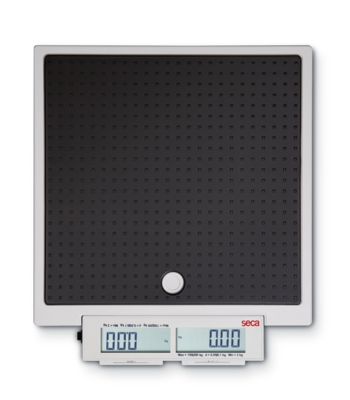
\includegraphics{images/seca874.png}
\caption{SECA scale model 874}
\end{figure}

B. General use, care and maintenance of SECA tared scales

\begin{enumerate}
\def\labelenumi{\arabic{enumi}.}
\item
  Place the scale on a hard, level surface (wood, concrete, or firm
  earth). Soft or uneven surfaces may cause small errors in weighing. It
  is therefore advisable that each survey team are provided with a
  wooden plank that can be laid on top of unlevel ground as a way to
  even out the surface. The plank should be big enough to cover a
  reasonable surface and sturdy enough to carry the weight of the scale
  and those being weighed.
\item
  The scale will not function correctly if it becomes too warm. It is
  best to use the scale in the shade, or indoors. If the scale becomes
  hot and does not work correctly, place it in a cooler area and wait 15
  minutes before using again.
\item
  The scale must adjust to changes in temperature. If the scale is moved
  to a new site with a different temperature, wait for 15 minutes before
  using the scale again. It is advisable to test the scale before every
  measurement when the scale is moved and operated in extreme weather
  conditions.
\item
  The scale must be tested every single day of fieldwork. This is best
  done using a labelled standard weight of 2.5 - 5.0 kg. This can be
  purchased locally, but must be tested initially to ensure that the
  indicated weight is accurate. Record the results of the daily test of
  the scale, including the date and weight. Using other types of
  standard weights is possible, but is not recommended. Some surveys
  have in the past used filled water bottles for testing, but as water
  or other liquids evaporate, this technique is flawed. Sand is a viable
  alternative, but only if labelled weights are not available.
\item
  Handle the scale carefully:

  \begin{itemize}
  \tightlist
  \item
    Do not drop or bump the scale.
  \item
    Do not weigh loads with a total weight of more than 150 kg.
  \item
    Do not store the scale in direct sunlight or other hot places.
  \item
    Protect the scale against excess humidity or wetness.
  \item
    Do not use the scale at temperatures below 10º C or above 45º C.
  \end{itemize}
\item
  The scale is battery-powered. Around 120,000 weighings can be
  performed with a fresh set of batteries.
\end{enumerate}

\hypertarget{anthro3}{%
\chapter{Anthropometric measurement standardisation
test}\label{anthro3}}

This chapter provides detailed instructions on how to carry out an
anthropometric measurement standardisation test as part of a training
process in preparation for a nutrition survey.

\bibliography{book.bib}


\end{document}
